\newcommand{\tttt}{Vectoren}
\newcommand{\dddd}{Datum 1}

\documentclass{article}
\usepackage[utf8]{inputenc}
\usepackage{hyperref}

\usepackage{listings}
\usepackage{color}
\usepackage{amsmath}
\usepackage{wrapfig}
\usepackage{graphicx}
\graphicspath{ {./images/} }
\usepackage{tikz}

\definecolor{mygreen}{rgb}{0,0.6,0}
\definecolor{mygray}{rgb}{0.5,0.5,0.5}
\definecolor{mymauve}{rgb}{0.58,0,0.82}

\lstset{ %
  backgroundcolor=\color{white},   % choose the background color
  basicstyle=\footnotesize,        % size of fonts used for the code
  breaklines=true,                 % automatic line breaking only at whitespace
  captionpos=b,                    % sets the caption-position to bottom
  commentstyle=\color{mygreen},    % comment style
  escapeinside={\%*}{*)},          % if you want to add LaTeX within your code
  keywordstyle=\color{blue},       % keyword style
  stringstyle=\color{mymauve},     % string literal style
  numbers=left,               % Ort der Zeilennummern
  language=java,
}

\newcommand{\myhref}[2]{\href{#1}{#2}\\\texttt{#1}}

\begin{document}

\title{\tttt}
\author{Steven Bronsveld}

\maketitle
\section{Gegevens}

\subsection{Algemene bronnen}
\begin{itemize}
    \item \myhref{http://www.github.com/StevenBrons/Processing}{GitHub Pagina} 
    \item \myhref{https://natureofcode.com/book}{Nature of Code boek} 
    \item \myhref{https://www.youtube.com/user/shiffman/playlists?view=50\&sort=dd\&shelf\_id=2}{Processing Basic tutorial}
\end{itemize}


\newpage


\section{Leerdoelen}
\begin{itemize}
	\item Omgaan met de \texttt{PVector} class
\end{itemize}

\section{Vectoren}
Omdat het onhandig is om telkens twee argumenten mee te moeten geven voor een positie op het scherm \texttt{int x, int y} en we een betere manier nodig hebben om met co\"ordinaten om te gaan bestaat er in Processing de \texttt{PVector} class.

\subsection{[optioneel] Vectoren in de wiskunde}
Een vector is een verzameling van meerdere variabelen. Wij zullen ons alleen maar bezig houden met 2 dimensionale vectoren van \texttt{x,y} co\"ordinaten.
Een vector wordt als volgt genoteerd: 
$$
\vec{v}=
\begin{pmatrix}
2\\ 
3
\end{pmatrix}
$$
Er zijn een paar rekenregels, die erg voor de hand liggen als je bedenkt dat een vector gewoon een verzameling van twee co\"ordinaten is:
$$
\begin{pmatrix}
a\\ 
b
\end{pmatrix}
+
\begin{pmatrix}
c\\ 
d
\end{pmatrix}
=
\begin{pmatrix}
a + c\\ 
b + d
\end{pmatrix}
$$
$$
a * 
\begin{pmatrix}
b\\ 
c
\end{pmatrix}
=
\begin{pmatrix}
a*b\\ 
a*c
\end{pmatrix}
$$
De tweede rekenregel heet \textit{scalaire vermenigvuldiging}. Dit geeft het uitrekken of inkrimpen van een vector weer. Dit is makkelijker te zien als we de vectoren als pijltjes (of natuurkundige krachten) tekenen:\\
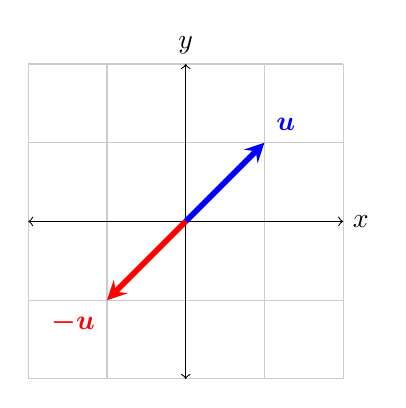
\begin{tikzpicture}
  \draw[thin,gray!40] (-2,-2) grid (2,2);
  \draw[<->] (-2,0)--(2,0) node[right]{$x$};
  \draw[<->] (0,-2)--(0,2) node[above]{$y$};
  \draw[line width=2pt,blue,-stealth](0,0)--(1,1) node[anchor=south west]{$\boldsymbol{u}$};
  \draw[line width=2pt,red,-stealth](0,0)--(-1,-1) node[anchor=north east]{$\boldsymbol{-u}$};
\end{tikzpicture}
\subsubsection{Opdrachten}
\begin{enumerate}
	\item Teken de optelling van $\begin{pmatrix}2\\1\end{pmatrix}+\begin{pmatrix}-1\\3\end{pmatrix}$
	\item Bereken $2*((3*\vec{a})+\vec{b})$ met $\vec{a}=\begin{pmatrix}1\\2\end{pmatrix}$ en $\vec{b} = \begin{pmatrix}-1\\2\end{pmatrix}$
	\item Bepaal het midden tussen $\vec{a}$ en $\vec{b}$. (We zoeken dus een algemene formule voor het midden tussen twee vectoren).
	\item Bereken het punt op $\frac{2}{3}$ afstand tussen $\vec{a}$ en $\vec{b}$ (Wederom zoeken we dus een algemene formule).
\end{enumerate}

\subsection{PVector}
Processing heeft de class \texttt{PVector}, met daarin een heleboel handige methods, zie \texttt{https://processing.org/reference/PVector.html}
\begin{lstlisting}
	void setup() {
		PVector v1 = new PVector(3,2);
		PVector v2 = v1.copy();
		v1.add(v2);
		v2.sub(new PVector(1,1));
		v1.mult(3);
		drawDot(v1);
		drawDot(v2);
	}
	
	void drawDot(PVector v) {
		circle(v.x,v.y,5);
	}
\end{lstlisting}
\textbf{Let op! De oorsprong (0,0) zit bij computers links boven, en niet links onder zoals bij de meeste wiskundige grafieken! De y-as is als het ware gespiegeld!}\\
Op welke co\"ordinaten tekent dit stukje code een stip?
Schrijf je antwoord in een comment van je sketch:
\begin{lstlisting}
	// dit is een comment
	// alles na de twee slashes word door 
	// Processing overgeslagen!
\end{lstlisting}


\section{Inleveren}
Als je klaar bent met de hele opdracht kun je deze naar je \textit{repository} \texttt{pushen}.



\end{document}
